
\section{Integrales y Primitivas}

\textcolor{red}{Referencia: Diferencial, semanas 5}

\subsection{Primitivas}

\begin{definicion}
	Una función $F$ continua en un intervalo $I\subseteq\R$ y derivable en $Int(I)$ se llama \textbf{primitiva} (o \textbf{integral indefinida}) de una función $f$ sobre $I$ ssi $\forall x \in Int(I)$, $F'(x) = f(x)$. 
	
	\textbf{Notación:} 
	\begin{itemize}
		\item Al conjunto de todas las primitivas de $f$ lo denotamos por $\displaystyle \int f$.
				
		\item Si $F$ es una primitiva de $f$, entonces en lugar de escribir $F \in \displaystyle f$, escribiremos $F =\displaystyle \int f$. 
		
		\item Es habitual además utilizar la notación clásica: 
		$$ \int f(x) dx = F(x) + c $$ 
		Donde $dx$ corresponde a un símbolo que identifica la variable. 
	\end{itemize} 
\end{definicion}

\begin{nota}
	Notemos que: 
	\begin{itemize}
		\item 	Sean $F_1$ y $F_2$ dos primitivas de una misma función $f$ sobre $I$. Entonces: 
		$$ F_1 ' = f = F_2 ' \quad \Longrightarrow \quad (F_1  - F_2) ' = 0 $$ 
		Luego: 
		$$ F_1 - F_2 = \text{cte} $$ 
		Es decir, \textbf{primitivas de una misma función difieren, a lo más, en una constante.}
		
		\item Si $F$ es una primitiva de $f$, entonces la función $F + c$, con $c\in \R$, es otra primitiva de $f$. 
		
		Es decir, \textbf{dada una primitiva de una función, puedo encontrar infinitas primitivas que solo difieren en una constante}. 
	\end{itemize}
\end{nota}

\begin{proposicion}
	Algunas primitivas que se obtienen fácilmente a partir del conocimiento adquirido en el capítulo de derivadas son las siguientes: 
	\begin{itemize}
		\item $\displaystyle \int x^n dx = \dfrac{x^{n+1}}{n+1} + c$, $\forall n \neq -1$. 
		\item $\displaystyle \int \dfrac{dx}{x} = ln (x) + c $
		\item $\displaystyle \int \sin(x)dx = - \cos(x) + c $
		\item $\displaystyle \int \cos(x)dx = \sin(x) + c$
		\item $\displaystyle \int e^{ax}dx = \dfrac{1}{a} e^{ax} + c$
	\end{itemize}
\end{proposicion}

\begin{proposicion}
	De la definición anterior se obtiene además que: 
	\begin{itemize}
		\item $\displaystyle \int f'(x) dx = f(x) + c$
		\item $\dfrac{d}{dx} \displaystyle \int f(x) dx = f(x)$
		\item $\displaystyle \int f' = f + c $
		\item $\displaystyle \left(\int f \right)' = f$ 
	\end{itemize}
\end{proposicion}

\begin{proposicion}
	$\displaystyle \int$ es un operador lineal, es decir: 
	\begin{itemize}
		\item $\displaystyle \int f \pm g = \int f \pm \int g$
		\item $\displaystyle \int \alpha f = \alpha \int f$, $\forall \alpha \in \R$
	\end{itemize}
\end{proposicion}

\begin{proof}
	Sean $(F + c) \in \displaystyle \int f$, $(G + k) \in \displaystyle \int g$ y $\alpha \in \R$. Se tiene que: 
	$$  F ' = f, \quad (\alpha F)' = \alpha f, \quad G' = g $$
	Luego: 
	$$ (F \pm G)' = (f \pm g) , \quad (\alpha F)' = \alpha f $$ 
	De lo anterior se concluye. 	
\end{proof}

\begin{teorema}
	\textbf{(Cambio de variable)} Si $u = g(x)$, entonces: 
	$$ \displaystyle \int f(u) du = \int (f \circ g)(x) \cdot g'(x) dx $$ 
	O equivalentemente: 
	$$ \displaystyle \int f = \int (f \circ g) \cdot g' $$ 
\end{teorema}

\begin{proof}
	Sea $F$ una primitiva de $f$, es decir, $F'(u) = f(u)$. Como $u = g(x)$, entonces $F(u) = (F \circ g)(x)$. 
	
	Calculemos: 
	$$ (F \circ g)(x) =  F'(g(x))\cdot g'(x) = f(g(x))\cdot g'(x) $$ 
	Por lo tanto, $(F \circ g)$ es una primitiva de $f(g(x))g'(x)$. 
	Es decir: 
	$$ F(u) = \int f(u)\quad \wedge \quad (F \circ g) = \int (f \circ g ) \cdot g'$$ 
	Pero $F(u) = (F\circ g) (x)$, luego $\displaystyle \int f(u) du = \int (f \circ g) (x) g'(x) dx$. 
\end{proof}

\begin{teorema}
	\textbf{(Fórmula de integración por partes)}
	Sean $u$ y $v$ dos funciones de $x$, entonces: 
	$$ \int u(x) v'(x) dx = u(x) v(x) - \int u'(x) v(x) dx $$ 
	O equivalentemente: 
	$$ \int u \cdot v' = u \cdot v - \int u' v $$ 
\end{teorema}

\begin{proof}
	Recordemos primero que: 
	$$ (u(x)v(x))' = u'(x) v(x) + u(x) v'(x) $$
	Gracias a que la primitiva es un operador lineal: 
	$$ u(x) v(x) = \int u'(x) v(x) dx + \int u(x) v'(x) dx $$ 
	Reordenando los términos se obtiene la fórmula de integración por partes. 
\end{proof}

\subsection{Integral de Riemann}

A modo de motivación, consideramos la función $f(x) = x^2$. Lo que queremos hacer, es calcular el área bajo la curva que describe la función $f$, entre $x=a\geq 0$ y $x=b>0$ para valores fijos de $a$ y $b$. 

\begin{center}
	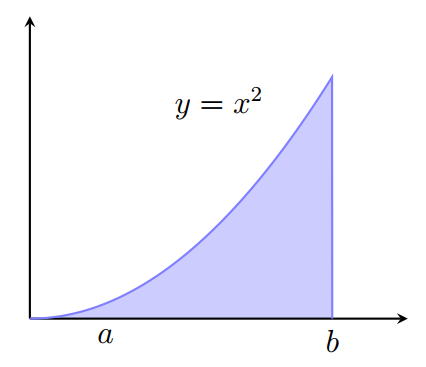
\includegraphics[scale=0.6]{figuras/capitulo1/06-integrales/motivacion.png}
\end{center}

\begin{definicion}
	\textbf{(Partición de un intervalo)} El conjunto $P = \{ x_0, x_1, ... , x_n\}$ es una partición del intervalo $[a, b]$ si $a = x_0 < x_1 < ... < x_n = b$. 
	
	Si $P$ es una partición de $[a,b]$, denotamos por $|P|$ al real: 
	$$ |P| = \max \{ x_i - x_{i-1} : i = 1, ... , n \} $$ 
\end{definicion}


\begin{definicion}
	\textbf{(Sumas superiores e inferiores)} Sea $f$ una función definida y acotada en $[a, b]$. Sea $P = \{ x_0, x_1, ... , x_n\}$ una partición de $[a, b]$. Como $f$ es acotada en $[a, b]$, también lo es en cada intervalo $I_i = [ x_{i-1}, x_i]$, $\forall i = 1, ..., n$. Por lo tanto, podemos definir: 
	$$ m_i(f) = inf\{f(x) : x \in [ x_{i-1}, x_i]\}$$ 
	$$ M_i(f) = sup\{f(x) : x \in [ x_{i-1}, x_i]\}$$ 
	Se definen las sumas: 
	$$ S(f, P) = \sum_{i=1}^n M_i(f) (x_i - x_{i-1})$$
	$$ s(f, P) = \sum_{i=1}^n m_i(f) (x_i - x_{i-1})$$
	Que llamamos \textbf{suma superior} y \textbf{suma inferior} de $f$ respecto de la partición $P$, respectivamente. 
\end{definicion}

\begin{nota}
	Es fácil ver que: 
	$$ m_i(f) \leq M_i (f) $$ 
	Y, por lo tanto: 
	$$ s(f, P) \leq S(f, P) $$ 
	Para cualquier función $f$ definida, continua y acotada en $[a, b]$. 
\end{nota}

\begin{definicion}
	\textbf{(Integrales superiores e inferiores)}
	\textcolor{red}{completar!}
\end{definicion}

\begin{definicion}
	contenidos...
\end{definicion}